\subsection{图的遍历}
\begin{frame}\ft{\subsecname}
  \begin{dingyi}
    从图中某一顶点出发访遍图中其余顶点,且使每一个顶点仅被访问一次,这一过程叫做图的遍历(\tf Traversing Graph)。
  \end{dingyi}
  图的遍历分为两种:
  \begin{itemize}
  \item 深度优先遍历
  \item 广度优先遍历
  \end{itemize}
\end{frame}


\subsection{\tf 深度优先遍历(Depth First Search, DFS)}
\begin{frame}\ft{\subsubsecname}
  \begin{figure}
    \centering
    \begin{tikzpicture}[scale=0.5,node distance=2cm,semithick,inner sep=1pt,bend angle=45]
%\draw[help lines] (-3,-3) grid (3,0);
\node[state]   (v1)                     {A};
\node[state]   (v2) [below left  of=v1] {B};
\node[state]   (v3) [below right of=v1] {F};
\node[state]   (v4) [below left  of=v2] {C};
\node[state]   (v5) [below       of=v1] {G};
\node[state]   (v6) [below right of=v3] {E};
\node[state]   (v7) [below right of=v5] {H};
\node[state]   (v8) [right       of=v4] {I};
\node[state]   (v9) [below       of=v7] {D};

\path
(v1) edge node{} (v2)
     edge node{} (v3)
(v2) edge node{} (v4)
     edge node{} (v5)
     edge node{} (v8)
(v3) edge node{} (v5)
     edge node{} (v6)
(v4) edge node{} (v8)
     edge node{} (v9)
(v5) edge node{} (v7)
     edge node{} (v9)
(v6) edge node{} (v7)
     edge node{} (v9)
(v7) edge node{} (v9)
(v8) edge node{} (v9);                     
\end{tikzpicture}

    \caption{深度优先遍历}    
  \end{figure}
\end{frame}

\begin{frame}\ft{\subsubsecname}
  \begin{itemize}
  \item \tf从A开始,标识已经走过,面前有两条路,即通项B和F。定一个规则,\blue{在没有碰到重复顶点的情况下,始终往右手边走(简称“右手通行规则”),}于是走到了B。\\[0.1in]%\pause
  \item \tf此时发现有三个分支,分别通向C、I、G,由右手通行规则,走到了C。\\[0.1in]%\pause
  \item \tf又有两个分支,分别通项I、D,由右手通行规则,走到了D。\\[0.1in]%\pause
  \item \tf接着有四个分支,分别通向I、G、H和E,由右手通行规则,走到了E。\\[0.1in]%\pause
  \item \tf然后只能通向F,若再由右手通行规则,会走回到A,但A已经走过,只能退回到F,走向从右数的第二个通道,到达G。\\[0.1in]%\pause
  \item 接着有三条通道,发现B和D已经走过,于是走到H,再观察H的两条通道D和E,发现已经走过。
  \end{itemize}
\end{frame}


\begin{frame}\ft{\subsubsecname}
  \begin{wenti}
    至此,我们是否已经遍历了所有顶点呢?
  \end{wenti}
  %\pause 
  没有。因为可能还有很多分支的顶点我们没有走过,所以我们需原路返回。

\end{frame}


\begin{frame}\ft{\subsubsecname}
  \begin{itemize}
  \item \tf在H处,再无通道没走过,返回至G,也再无未走过通道,返回至F,没有通道,返回至E,也无未走过通道,返回至D。\\[0.1in]%\pause 
  \item \tf 发现还有I没走过,这是新顶点,进行标记。继续返回,直到返回到A,这样便可以确认已经完成遍历任务,找到了所有9个顶点。
  \end{itemize}
\end{frame}

\begin{frame}\ft{\subsubsecname}
  \begin{figure}
    \centering
    \begin{tikzpicture}[scale=0.5,node distance=2cm,semithick,inner sep=1pt,bend angle=45]
  %\draw[help lines] (-3,-3) grid (3,0);
  \node[state]   (A)                    {A};
  \node[state]   (B) [below left  of=A] {B};
  \node[state]   (F) [below right of=A] {F};
  \node[state]   (C) [below left  of=B] {C};
  \node[state]   (G) [below       of=A] {G};
  \node[state]   (E) [below right of=F] {E};
  \node[state]   (H) [below right of=G] {H};
  \node[state]   (I) [right       of=C] {I};
  \node[state]   (D) [below       of=H] {D};

  \path
  (A) edge  (B) edge  (F)
  (B) edge  (C) edge  (G) edge  (I)
  (F) edge  (G) edge  (E)
  (C) edge  (I) edge  (D)
  (G) edge  (H) edge  (D)
  (E) edge  (H) edge  (D)
  (H) edge  (D)
  (I) edge  (D);

  \pause 
  \draw[->,>=latex',red] (A)to[bend right=8](B); \pause 
  \draw[->,>=latex',red] (B)to[bend right=8](C); \pause 
  \draw[->,>=latex',red] (C)to[bend right=8](D); \pause 
  \draw[->,>=latex',red] (D)to[bend right=8](E); \pause 
  \draw[->,>=latex',red] (E)to[bend right=8](F); \pause
  \draw[->,>=latex',red,densely dashed] (F)to[bend right=8](A); \pause
  \draw[->,>=latex',red,densely dashed] (A)to[bend right=8](F); \pause
  \draw[->,>=latex',red] (F)to[bend right=8](G); \pause
  \draw[->,>=latex',red,densely dashed] (G)to[bend right=8](B); \pause
  \draw[->,>=latex',red,densely dashed] (B)to[bend right=8](G); \pause
  \draw[->,>=latex',red,densely dashed] (G)to[bend right=8](D); \pause
  \draw[->,>=latex',red,densely dashed] (D)to[bend right=8](G); \pause
  \draw[->,>=latex',red] (G)to[bend right=8](H); \pause
  \draw[->,>=latex',red,densely dashed] (H)to[bend right=8](D); \pause
  \draw[->,>=latex',red,densely dashed] (D)to[bend right=8](H); \pause
  \draw[->,>=latex',red,densely dashed] (H)to[bend right=8](E); \pause
  \draw[->,>=latex',red,densely dashed] (E)to[bend right=8](H); \pause
  \draw[->,>=latex',blue](H)to[bend right=8](G); \pause
  \draw[->,>=latex',blue](G)to[bend right=8](F); \pause
  \draw[->,>=latex',blue](F)to[bend right=8](E); \pause
  \draw[->,>=latex',blue](E)to[bend right=8](D); \pause
  \draw[->,>=latex',red] (D)to[bend right=8](I); \pause
  \draw[->,>=latex',red,densely dashed] (I)to[bend right=8](B); \pause
  \draw[->,>=latex',red,densely dashed] (B)to[bend right=8](I); \pause
  \draw[->,>=latex',red,densely dashed] (I)to[bend right=8](C); \pause
  \draw[->,>=latex',red,densely dashed] (C)to[bend right=8](I); \pause
  \draw[->,>=latex',blue](I)to[bend right=8](D); \pause
  \draw[->,>=latex',blue](D)to[bend right=8](C); \pause
  \draw[->,>=latex',blue](C)to[bend right=8](B); \pause
  \draw[->,>=latex',blue](B)to[bend right=8](A); \pause
\end{tikzpicture}

    \caption{深度优先遍历}    
  \end{figure}
\end{frame}

\begin{frame}\ft{\subsubsecname}
  \begin{dingyi}[连通图的深度优先遍历]
    从图中某个顶点$v$出发,访问此顶点,然后从$v$的未被访问的邻接点出发深度优先遍历图,直到图中所有与$v$有路径相同的顶点都被访问到。
  \end{dingyi}
\end{frame}

\begin{frame}\ft{\subsubsecname}
  \begin{dingyi}[非连通图的深度优先遍历]
    只需要对它的连通分量分别进行深度优先遍历,即在先前一个顶点进行一次深度优先遍历后,若图中尚有顶点未被访问,则另选图中一个未曾被访问的顶点作为起始点,重复上述过程,直到图中所有顶点都被访问到为止。
  \end{dingyi}
\end{frame}

\begin{frame}\ft{\subsecname}
  \lstinputlisting[
    language=C,
    title=\tf dfs.c (adjacent matrix),
    numbers=left,
    numberstyle=\tiny,
    frame=tb,
    xleftmargin=3pt,
    linerange={20-30},
  ]{Chapters/Ch06/Code/adjmatrix/adjmatrix.c}
\end{frame}

\begin{frame}\ft{\subsubsecname}
  \lstinputlisting[
    language=C,
    title=\tf dfstraverse.c (adjacent matrix),
    numbers=left,
    numberstyle=\tiny,
    frame=tb,
    xleftmargin=3pt,
    linerange={32-39},
  ]{Chapters/Ch06/Code/adjmatrix/adjmatrix.c}  
\end{frame}


\begin{frame}\ft{\subsecname}
  \lstinputlisting[
    language=C,
    title=\tf dfs.c (adjacent list),
    numbers=left,
    numberstyle=\tiny,
    frame=tb,
    xleftmargin=3pt,
    linerange={29-39},
  ]{Chapters/Ch06/Code/adjlist/adjlist.c}
\end{frame}

\begin{frame}\ft{\subsubsecname}
  \lstinputlisting[
    language=C,
    title=\tf dfstraverse.c  (adjacent list),
    numbers=left,
    numberstyle=\tiny,
    frame=tb,
    xleftmargin=3pt,
    linerange={41-48},
  ]{Chapters/Ch06/Code/adjlist/adjlist.c}  
\end{frame}


\subsection{\tf 广度优先遍历(Breadth First Search, BFS)}


\begin{frame}\ft{\subsubsecname}
  \begin{figure}
    \centering
    \begin{minipage}{0.45\textwidth}
    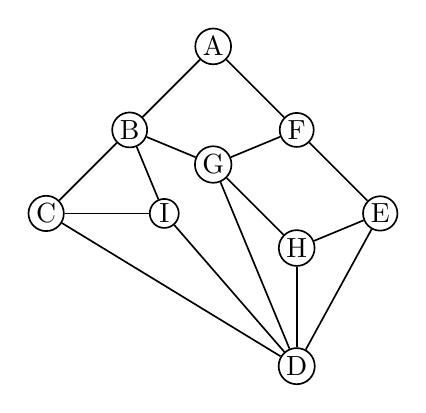
\begin{tikzpicture}[scale=0.25,node distance=1.5cm,semithick,inner sep=1pt,bend angle=45]
%\draw[help lines] (-3,-3) grid (3,0);
\node[circle,draw]   (v1)                     {\tf A};
\node[circle,draw]   (v2) [below left  of=v1] {\tf B};
\node[circle,draw]   (v3) [below right of=v1] {\tf F};
\node[circle,draw]   (v4) [below left  of=v2] {\tf C};
\node[circle,draw]   (v5) [below       of=v1] {\tf G};
\node[circle,draw]   (v6) [below right of=v3] {\tf E};
\node[circle,draw]   (v7) [below right of=v5] {\tf H};
\node[circle,draw]   (v8) [right       of=v4] {\tf I};
\node[circle,draw]   (v9) [below       of=v7] {\tf D};

\path
(v1) edge node{} (v2)
     edge node{} (v3)
(v2) edge node{} (v4)
     edge node{} (v5)
     edge node{} (v8)
(v3) edge node{} (v5)
     edge node{} (v6)
(v4) edge node{} (v8)
     edge node{} (v9)
(v5) edge node{} (v7)
     edge node{} (v9)
(v6) edge node{} (v7)
     edge node{} (v9)
(v7) edge node{} (v9)
(v8) edge node{} (v9);                     
\end{tikzpicture}
  
    \end{minipage} 
    \begin{minipage}{0.45\textwidth}
    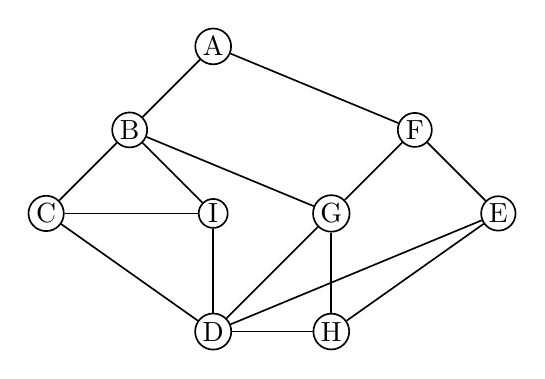
\begin{tikzpicture}[scale=0.25,node distance=1.5cm,semithick,inner sep=1pt,bend angle=45]
%\draw[help lines] (-3,-3) grid (3,0);
\node[circle,draw]   (A)                    {\tf A};
\node[]   (A1)[right of=A]       {};
\node[circle,draw]   (B) [below left  of=A] {\tf B};
\node[circle,draw]   (F) [below right of=A1]{\tf F};
\node[circle,draw]   (C) [below left  of=B] {\tf C};
\node[circle,draw]   (G) [below left  of=F] {\tf G};
\node[circle,draw]   (E) [below right of=F] {\tf E};
\node[circle,draw]   (H) [below       of=G] {\tf H};
\node[circle,draw]   (I) [below right of=B] {\tf I};
\node[circle,draw]   (D) [below       of=I] {\tf D};
                                              
\path
(A) edge node{} (B)
    edge node{} (F)
(B) edge node{} (C)
    edge node{} (G)
    edge node{} (I)
(F) edge node{} (G)
    edge node{} (E)
(C) edge node{} (I)
    edge node{} (D)
(G) edge node{} (H)
    edge node{} (D)
(E) edge node{} (H)
    edge node{} (D)
(H) edge node{} (D)
(I) edge node{} (D);                     
\end{tikzpicture}
  
    \end{minipage}    
    \caption{广度优先遍历}    
  \end{figure}
\end{frame}


%% \begin{frame}\ft{\subsubsecname}
%%   \begin{figure}
%%     \centering
%%     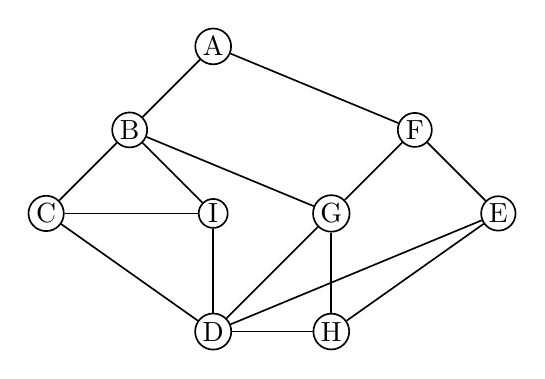
\begin{tikzpicture}[scale=0.25,node distance=1.5cm,semithick,inner sep=1pt,bend angle=45]
%\draw[help lines] (-3,-3) grid (3,0);
\node[circle,draw]   (A)                    {\tf A};
\node[]   (A1)[right of=A]       {};
\node[circle,draw]   (B) [below left  of=A] {\tf B};
\node[circle,draw]   (F) [below right of=A1]{\tf F};
\node[circle,draw]   (C) [below left  of=B] {\tf C};
\node[circle,draw]   (G) [below left  of=F] {\tf G};
\node[circle,draw]   (E) [below right of=F] {\tf E};
\node[circle,draw]   (H) [below       of=G] {\tf H};
\node[circle,draw]   (I) [below right of=B] {\tf I};
\node[circle,draw]   (D) [below       of=I] {\tf D};
                                              
\path
(A) edge node{} (B)
    edge node{} (F)
(B) edge node{} (C)
    edge node{} (G)
    edge node{} (I)
(F) edge node{} (G)
    edge node{} (E)
(C) edge node{} (I)
    edge node{} (D)
(G) edge node{} (H)
    edge node{} (D)
(E) edge node{} (H)
    edge node{} (D)
(H) edge node{} (D)
(I) edge node{} (D);                     
\end{tikzpicture}

%%     \caption{广度优先遍历}    
%%   \end{figure}
%% \end{frame}


\begin{frame}\ft{\subsubsecname}
  \lstinputlisting[
    language=C,
    title=\tf bfstraverse.c (adjacent matrix),
    numbers=left,
    numberstyle=\tiny,
    frame=tb,
    xleftmargin=3pt,
    linerange={42-52},
  ]{Chapters/Ch06/Code/adjmatrix/adjmatrix.c}  
\end{frame}


\begin{frame}\ft{\subsubsecname}
  \lstinputlisting[
    language=C,
    title=\tf bfstraverse.c (adjacent matrix),
    numbers=left,
    numberstyle=\tiny,
    frame=tb,
    firstnumber=12,
    xleftmargin=3pt,
    linerange={53-65},
  ]{Chapters/Ch06/Code/adjmatrix/adjmatrix.c}  
\end{frame}


\begin{frame}\ft{\subsubsecname}
  \lstinputlisting[
    language=C,
    title=\tf bfstraverse.c (adjacent list),
    numbers=left,
    numberstyle=\tiny,
    frame=tb,
    xleftmargin=3pt,
    linerange={51-62},
  ]{Chapters/Ch06/Code/adjlist/adjlist.c}  
\end{frame}


\begin{frame}\ft{\subsubsecname}
  \lstinputlisting[
    language=C,
    title=\tf bfstraverse.c (adjacent list),
    numbers=left,
    numberstyle=\tiny,
    frame=tb,
    firstnumber=12,
    xleftmargin=3pt,
    linerange={63-77},
  ]{Chapters/Ch06/Code/adjlist/adjlist.c}  
\end{frame}


\begin{frame}\ft{小结}
  对比深度优先遍历和广度优先遍历,时间复杂度一样,不同之处仅在于对顶点访问的顺序不同。由此可见两者在全图遍历上没有优劣之分,只是视不同情况选择不同的算法。
\end{frame}


\begin{frame}\ft{小结}
  若图的顶点和边非常多,不能在短时间内完成遍历,而遍历目的是为了寻找合适的顶点,那么选择何种遍历方式需仔细斟酌。\vspace{0.1in}

  \begin{itemize}
  \item 深度优先更适合目标明确,以找到目标为主要目的的情况。\\[0.1in]
  \item 广度优先更适合在不断扩大遍历范围时找到相对最优解的情况。
  \end{itemize}
\end{frame}
